\documentclass[11pt]{article}
\usepackage{amsfonts,amsmath,amssymb,amsthm}
\usepackage{array}
\usepackage{bm}
\usepackage{commath}
\usepackage{enumitem}
\usepackage{fancyhdr,fancyvrb}
\usepackage[letterpaper,text={7in,9in},centering]{geometry}
\usepackage[pdftex]{graphicx}
\usepackage{ifthen}
\usepackage{mathrsfs}
\usepackage{multicol}
\usepackage{pifont}
\usepackage{sectsty}
\usepackage{setspace}
\usepackage{stackrel}
\usepackage{stmaryrd}
\usepackage{tensor}
\usepackage{xspace}
\usepackage{natbib}
\usepackage{algorithm}
\usepackage{algpseudocode}

\pagestyle{fancy}
\fancyhead[RO]{Edward Gan \& Max Wang}

\sectionfont{\large}
\subsectionfont{\normalsize}

\newcommand{\Sequitur}{\textsc{Sequitur}\xspace}

\begin{document}
\bibliographystyle{plain}

\title{Squint: Lossy Hierarchical Compression on Symbol Streams}
\author{Edward Gan \& Max Wang}
\date{December 11, 2012}
\maketitle

\begin{abstract}
Grammar-based compression schemes like \Sequitur exploit repeated structures
in streams of symbolic data to achieve good compression ratios.
We develop a set of algorithms for improving upon Grammar-based compression 
schemes by allowing some loss in the compression. Although precise 
subsequences might be altered, in return we can simplify 
the grammars produced to obtain better ratios while still preserving
important syntatic patterns at both the micro and macro level.
\end{abstract}

\section{Introduction and Goals}
Many sources of data exhibit natural hierarchical structure. For instance,
english text often can be grouped well into sections, paragraphs, sentences, ...
all the way down to words and phonemes. Music too, consists of repeated motifs,
phrases, themes, and so on. Finally, computer code is so hierarchical that its
syntax can usually be put in BNF. This allows grammar-based compression schemes
to build up Context Free Grammars (CFGs) and achieve very good compression
ratios.

Taking a step back, in the image compression world there are both lossless and
lossy compression schemes. In certain situations, such as for low-pixel count
logos, one could use a lossless image compression scheme. In other situations
however, such as for textures and some photographs, the exact pixel values
are almost irrelevant compared to the overall gradients, colors, and structures
in the image, and one could use a lossy compression scheme like jpeg.

We believe it is valuable to bring some of the attitudes prevalent in image/
video compression to the world of hierarchical text compression. Better
compression ratios for text are possible. 

It may seem strange to allow a string such as "mind" to be lossily 
corrupted into ``rind'', but if one is more interested in recurrent 
structure in the text than in its precise meaning, these changes 
aren't important. For instance, if one is looking at a text in a foreign
language, one is more likely to pick up the texture, the repeated sounds,
some phrases that come up and the breaks between larger scale sections.
A change in a single letter probably wouldn't be noticed. Similarly,
when skimming through huge files, perhaps execution logs, one usually
first starts looking for patterns or things that stand out. Lorem ipsum
is a perfect example of a piece of ``text'' whose value lies in its texture
and sentence/paragraph structure, and we will come back to it again.

In this paper we develop 2 algorithms and implement a system for lossily
compressing text while preserving its hierarchical structures. The goal
was to preserve the feel of a text at both micro and macro levels. 
Since grammar-based compression schemes were designed to capture
these structures, we built
our system on top of the existing \Sequitur grammar inference algorithm. 
Starting with the CFG generated by a lossless grammar
inference algorithm, we repeatedly simplify it, throwing out details
along the way to emphasize repetitions. Our main contribution lies in the
development of 2 algorithms for ``simplifying'' CFG grammars while 
preserving their structure.

\section{Background}

TODO

\subsection{Grammar Compression}

TODO

\subsection{Lossy Compression}

TODO

Jpeg, Mpeg: using parts of previous frame to encode next frame, 
Fractal: Using self-similarity to encode

\section{Lossifier Algorithms}

\subsection{Motivation}

The scope of what we shall call a \emph{lossifier} algorithm is to take
an admissible CFG and simplify it. The output CFG should be smaller
than the input CFG but generate a string which preserves the
structure in the original string as much as possible. 

Building off the ideas in jpeg compression discussed
earlier, one idea for simplifying data is to look at a part
of the data and try to match it as closely as possible with an
existing set of primitives. In particular, just as with Mpeg and
fractal compression, to approximate one part of the grammar
we can use \emph{other parts of the grammar}. This is the seed for
both of our algorithms. Given a rule $S \rightarrow rhs$, we will
try to replace occurences of $S$ with other similar variables.

For example, consider the grammars in figure \ref{sred}.

\begin{figure}[t]
\centering
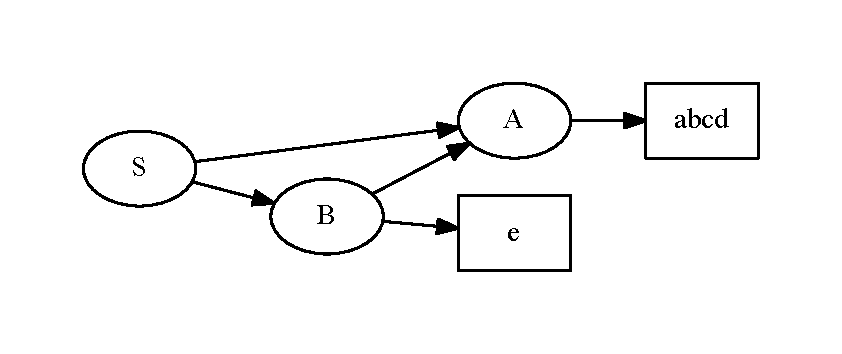
\includegraphics[scale=0.6]{sred1.pdf}
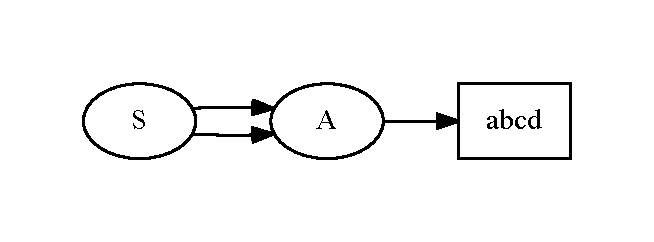
\includegraphics[scale=0.6]{sred2.pdf}
\caption{Grammar Simplification Example}
\label{sred}
\end{figure}

To simplify the grammar, it would make sense to replace B with A, since
they form two almost identical halves of S and are similar.

\subsection{Pair-Similarity}

To define whether two variables are \emph{similar}, we can look at their
expansions. Let $expand(rhs)$ denote the string of terminal symbols we get
when we recursively substitute all of the variables inside $rhs$. Then
$V_1 \rightarrow rhs_1$ and $V_2 \rightarrow rhs_2$ are similar when

$$\frac{levenshtein(expand(rhs_1),expand(rhs_2))}
        {max(len(expand(rhs_1)),len(expand(rhs_2)))} < \epsilon$$.

where $levenshtein$ is the levenstein edit distance between two strings.
For convenience we can define.

$$lsim(s1,s2) = \frac{levenshtein(s1,s2)}{max(len(s1),len(s2))}$$

The first algorithm takes the idea of variable similarity and uses it
to simplify the grammar sequentially as much as possible.

\begin{algorithm}
\caption{Similarity Lossifier Algorithm}
\label{sim_alg}
\begin{algorithmic}[1]
\Procedure{Lossify-Sim}{$g$} \Comment{Simplify grammar g}
  \While{there are similar variables to replace}
    \For{$var_1 \rightarrow rhs_1,\ var_2 \rightarrow rhs_2 \in g$}
      \State $str_{i} \gets expand(rhs_i)$
      \If{$lsim(str_{1},str_{2})<\epsilon$}
        \State replace the longer var with the shorter throughout $g$
        \State break
      \EndIf
    \EndFor
  \EndWhile
\EndProcedure
\end{algorithmic}
\end{algorithm}

\subsection{Clustering}

The previous algorithm updates the grammar sequentially, since each
variable replacement can have an effect on large parts of the grammar,
we will have to go through comparing all pairs again after the change.
An alternative algorithm would be to try to replace similar variables in
parallel. This would avoid many of the repeat pair-comparisons done in
\emph{Similarity}. In other words, the algorithm below makes puts 
similar variables
into equivalence class clusters, and then replaces them with a representative
all at once each iteration.

\begin{algorithm}
\caption{Cluster Lossifier Algorithm}
\label{cluster_alg}
\begin{algorithmic}[1]
\Procedure{Cluster-Sim}{$g$} \Comment{Simplify grammar g}
  \While{there are similar variables to replace}
    \State $clusters \gets ()$
    \For{$var_1 \rightarrow rhs_1 \in g$}
      \State blah
    \EndFor
  \EndWhile
\EndProcedure
\end{algorithmic}
\end{algorithm}

\subsection{Mathematical Analysis}
Runtime Analysis
No-loops proof

\section{Implementation}
Overview

\subsection{Grammar Reductions}
What is their purpose? Why do we want them? What are they?

\subsection{Data Structures and Optimizations}
Grammar Data Structure
Cluster Data Structure
Invariants Maintained
Core utility methods??
Linked Lists vs Arrays, Caching Expansions, Strings vs Symbols for expansion, Native Levenshtein

\section{Results}
\subsection{Illustrative Examples}
Qualitative, show off diagrams and detailed metrics for small examples
\subsection{Similarity vs Clustering}
Fixed compression ratio + fidelity comparison for different ratios
Show the runtime difference
\subsection{Grammar Reduction Impact}
\subsection{Larger Tests}

\section{Conclusions}
\subsection{Ratios and Fidelity}
\subsection{Future Work}

\nocite{*}

\bibliography{sources}

\end{document}
